\documentclass{beamer}

\usepackage{beamerthemesplit}

\title{An open hardware VJ platform}
\subtitle{Technical aspects}
\author{S\'ebastien Bourdeauducq}
\date{June 2009}

\begin{document}

\frame{
  \begin{figure}[H]
  
\includegraphics[height=18mm]{logo.eps}
  \end{figure}
  \titlepage
}

\section{Introduction}
\subsection{What we are speaking about}
\frame
{
  \frametitle{What we are speaking about}
A device for video performance artists (VJs)...
  \begin{itemize}
  \item inspired by the popular MilkDrop program for PCs
  \item with many interfaces: MIDI, DMX, can also do video mixing
  \item highly integrated
  \end{itemize}

At the frontier between...
  \begin{itemize}
  \item big computers with software to render visual effects
  \item and small, handy microcontroller boards you connect to anything\\(``Arduino'' is today's buzzword for those)
  \end{itemize}
}

\frame
{
  \frametitle{What is that MilkDrop thing?}
  \begin{figure}[H]
  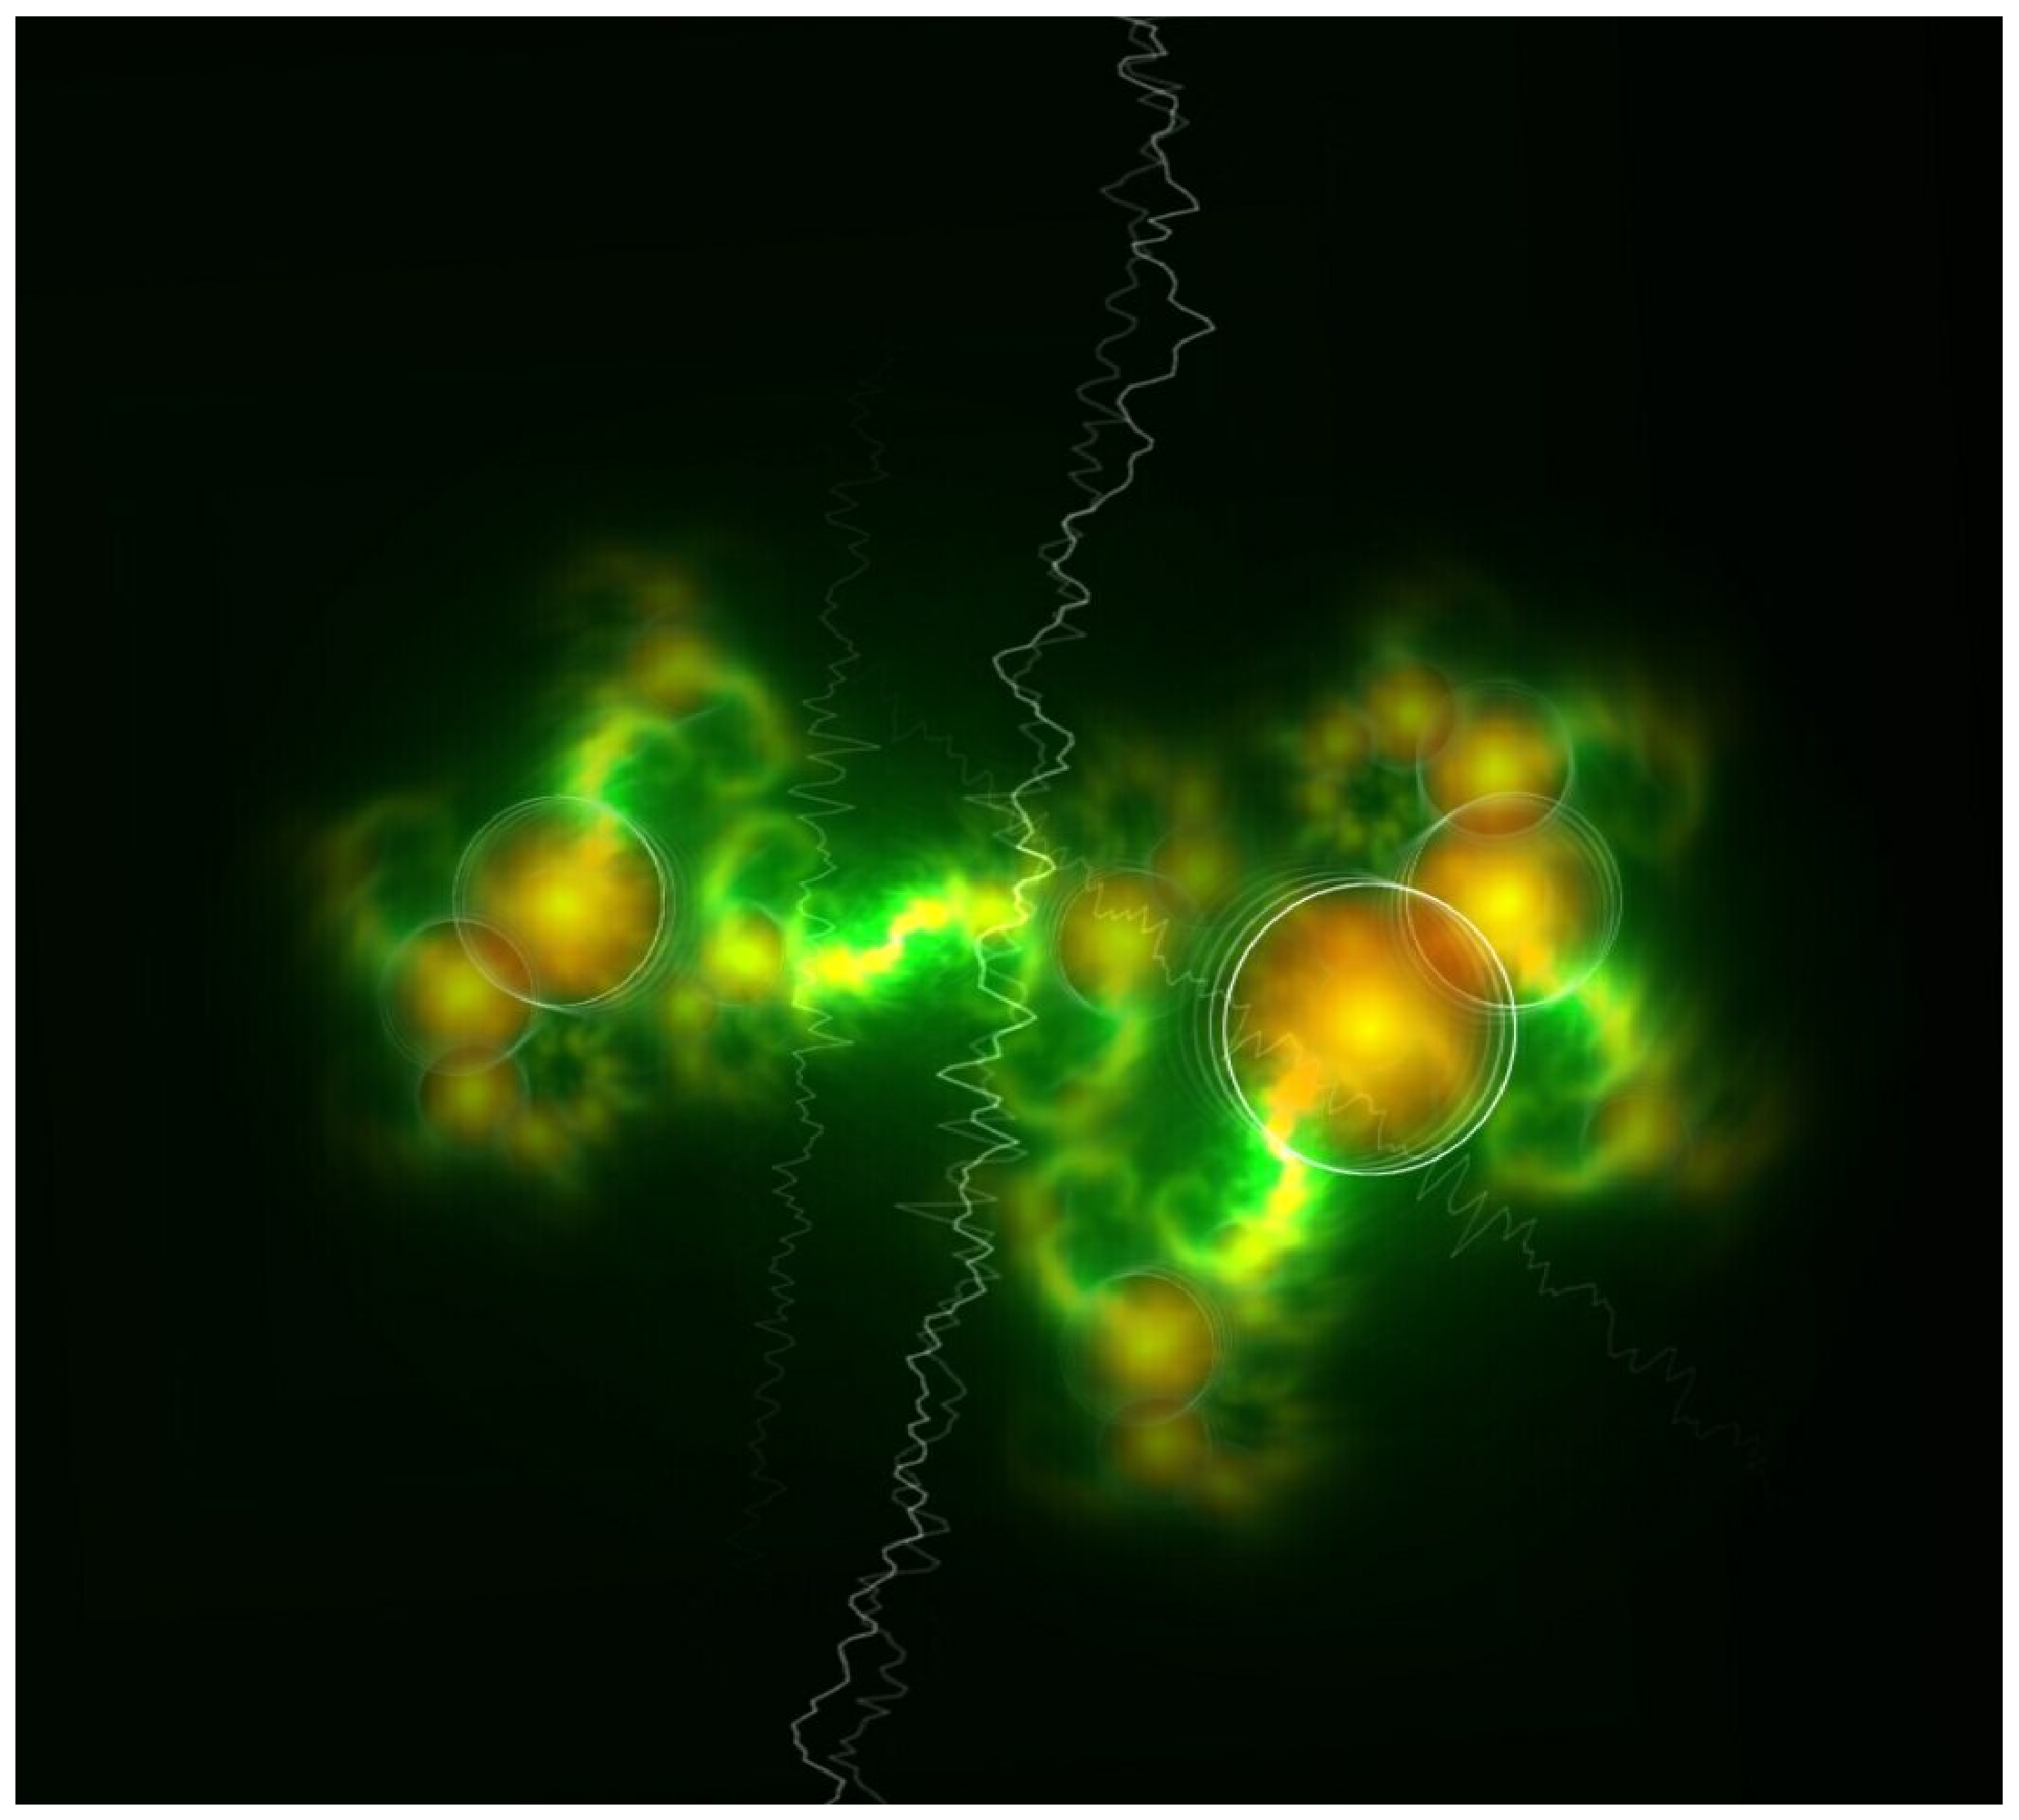
\includegraphics[height=58mm]{milkdrop1.eps}
  \end{figure}
}

\frame
{
  \frametitle{What is that MilkDrop thing?}
  \begin{figure}[H]
  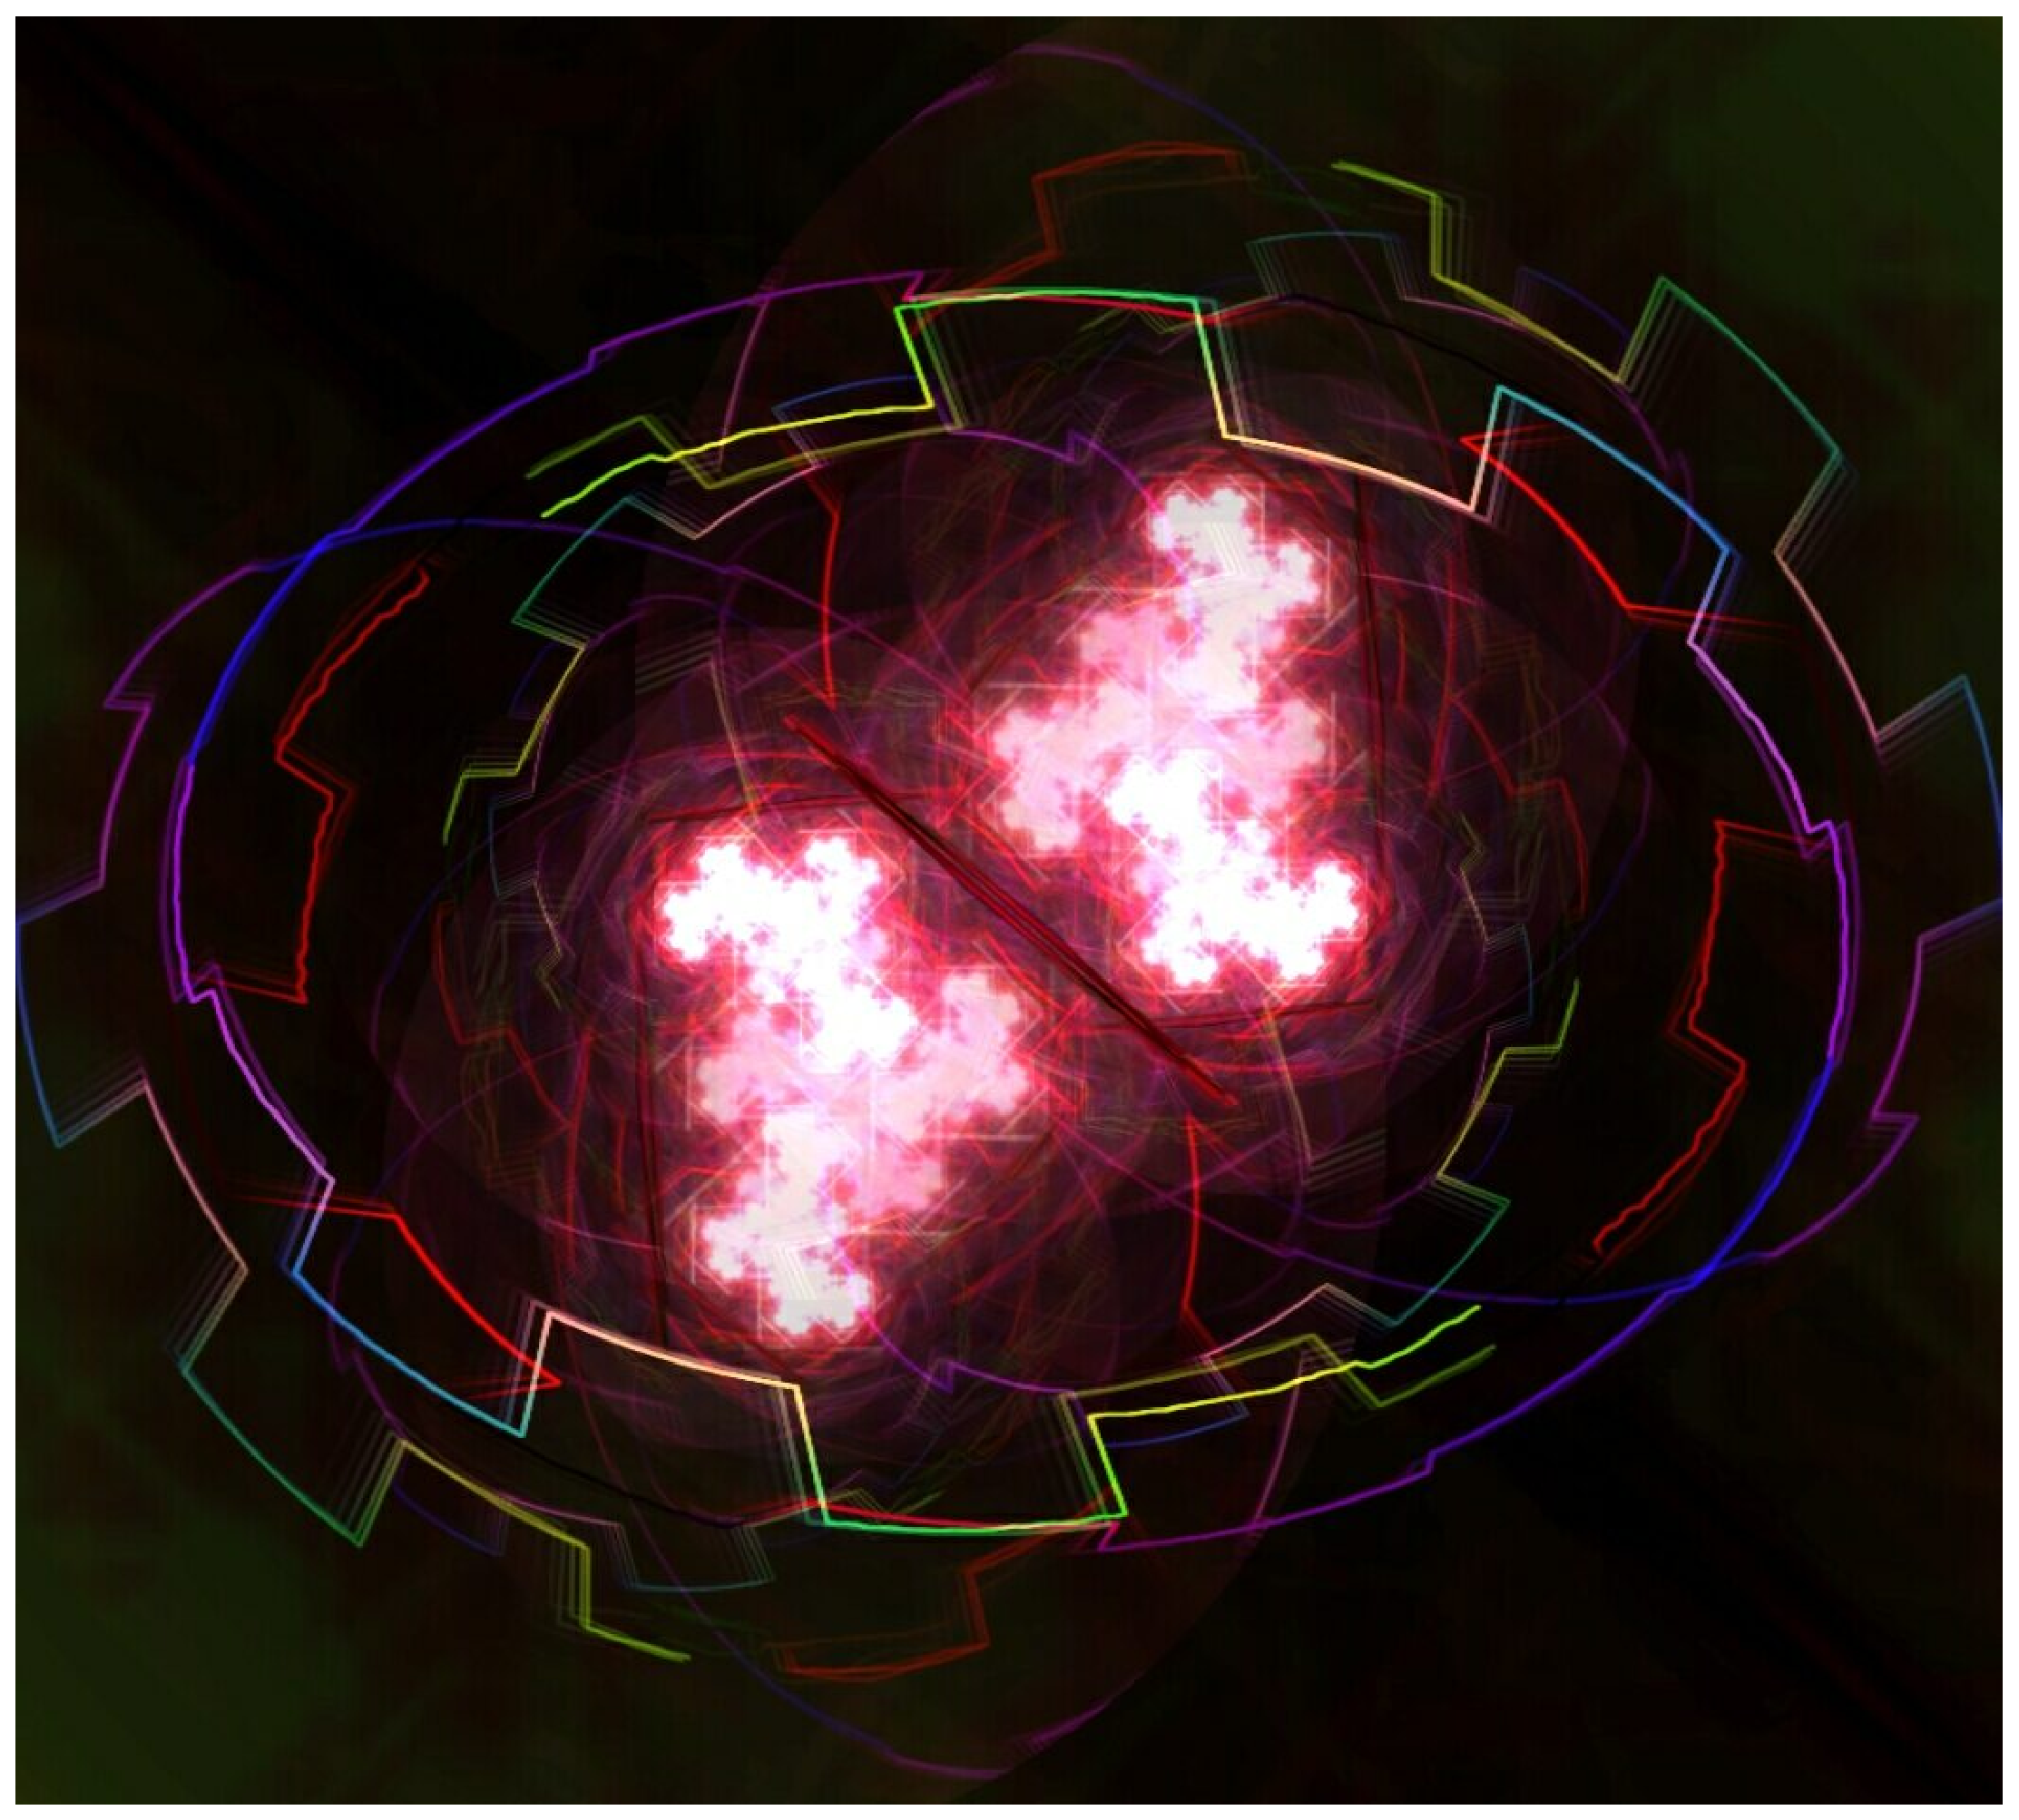
\includegraphics[height=58mm]{milkdrop2.eps}
  \end{figure}
}

\frame
{
  \frametitle{What is that MilkDrop thing?}
  \begin{figure}[H]
  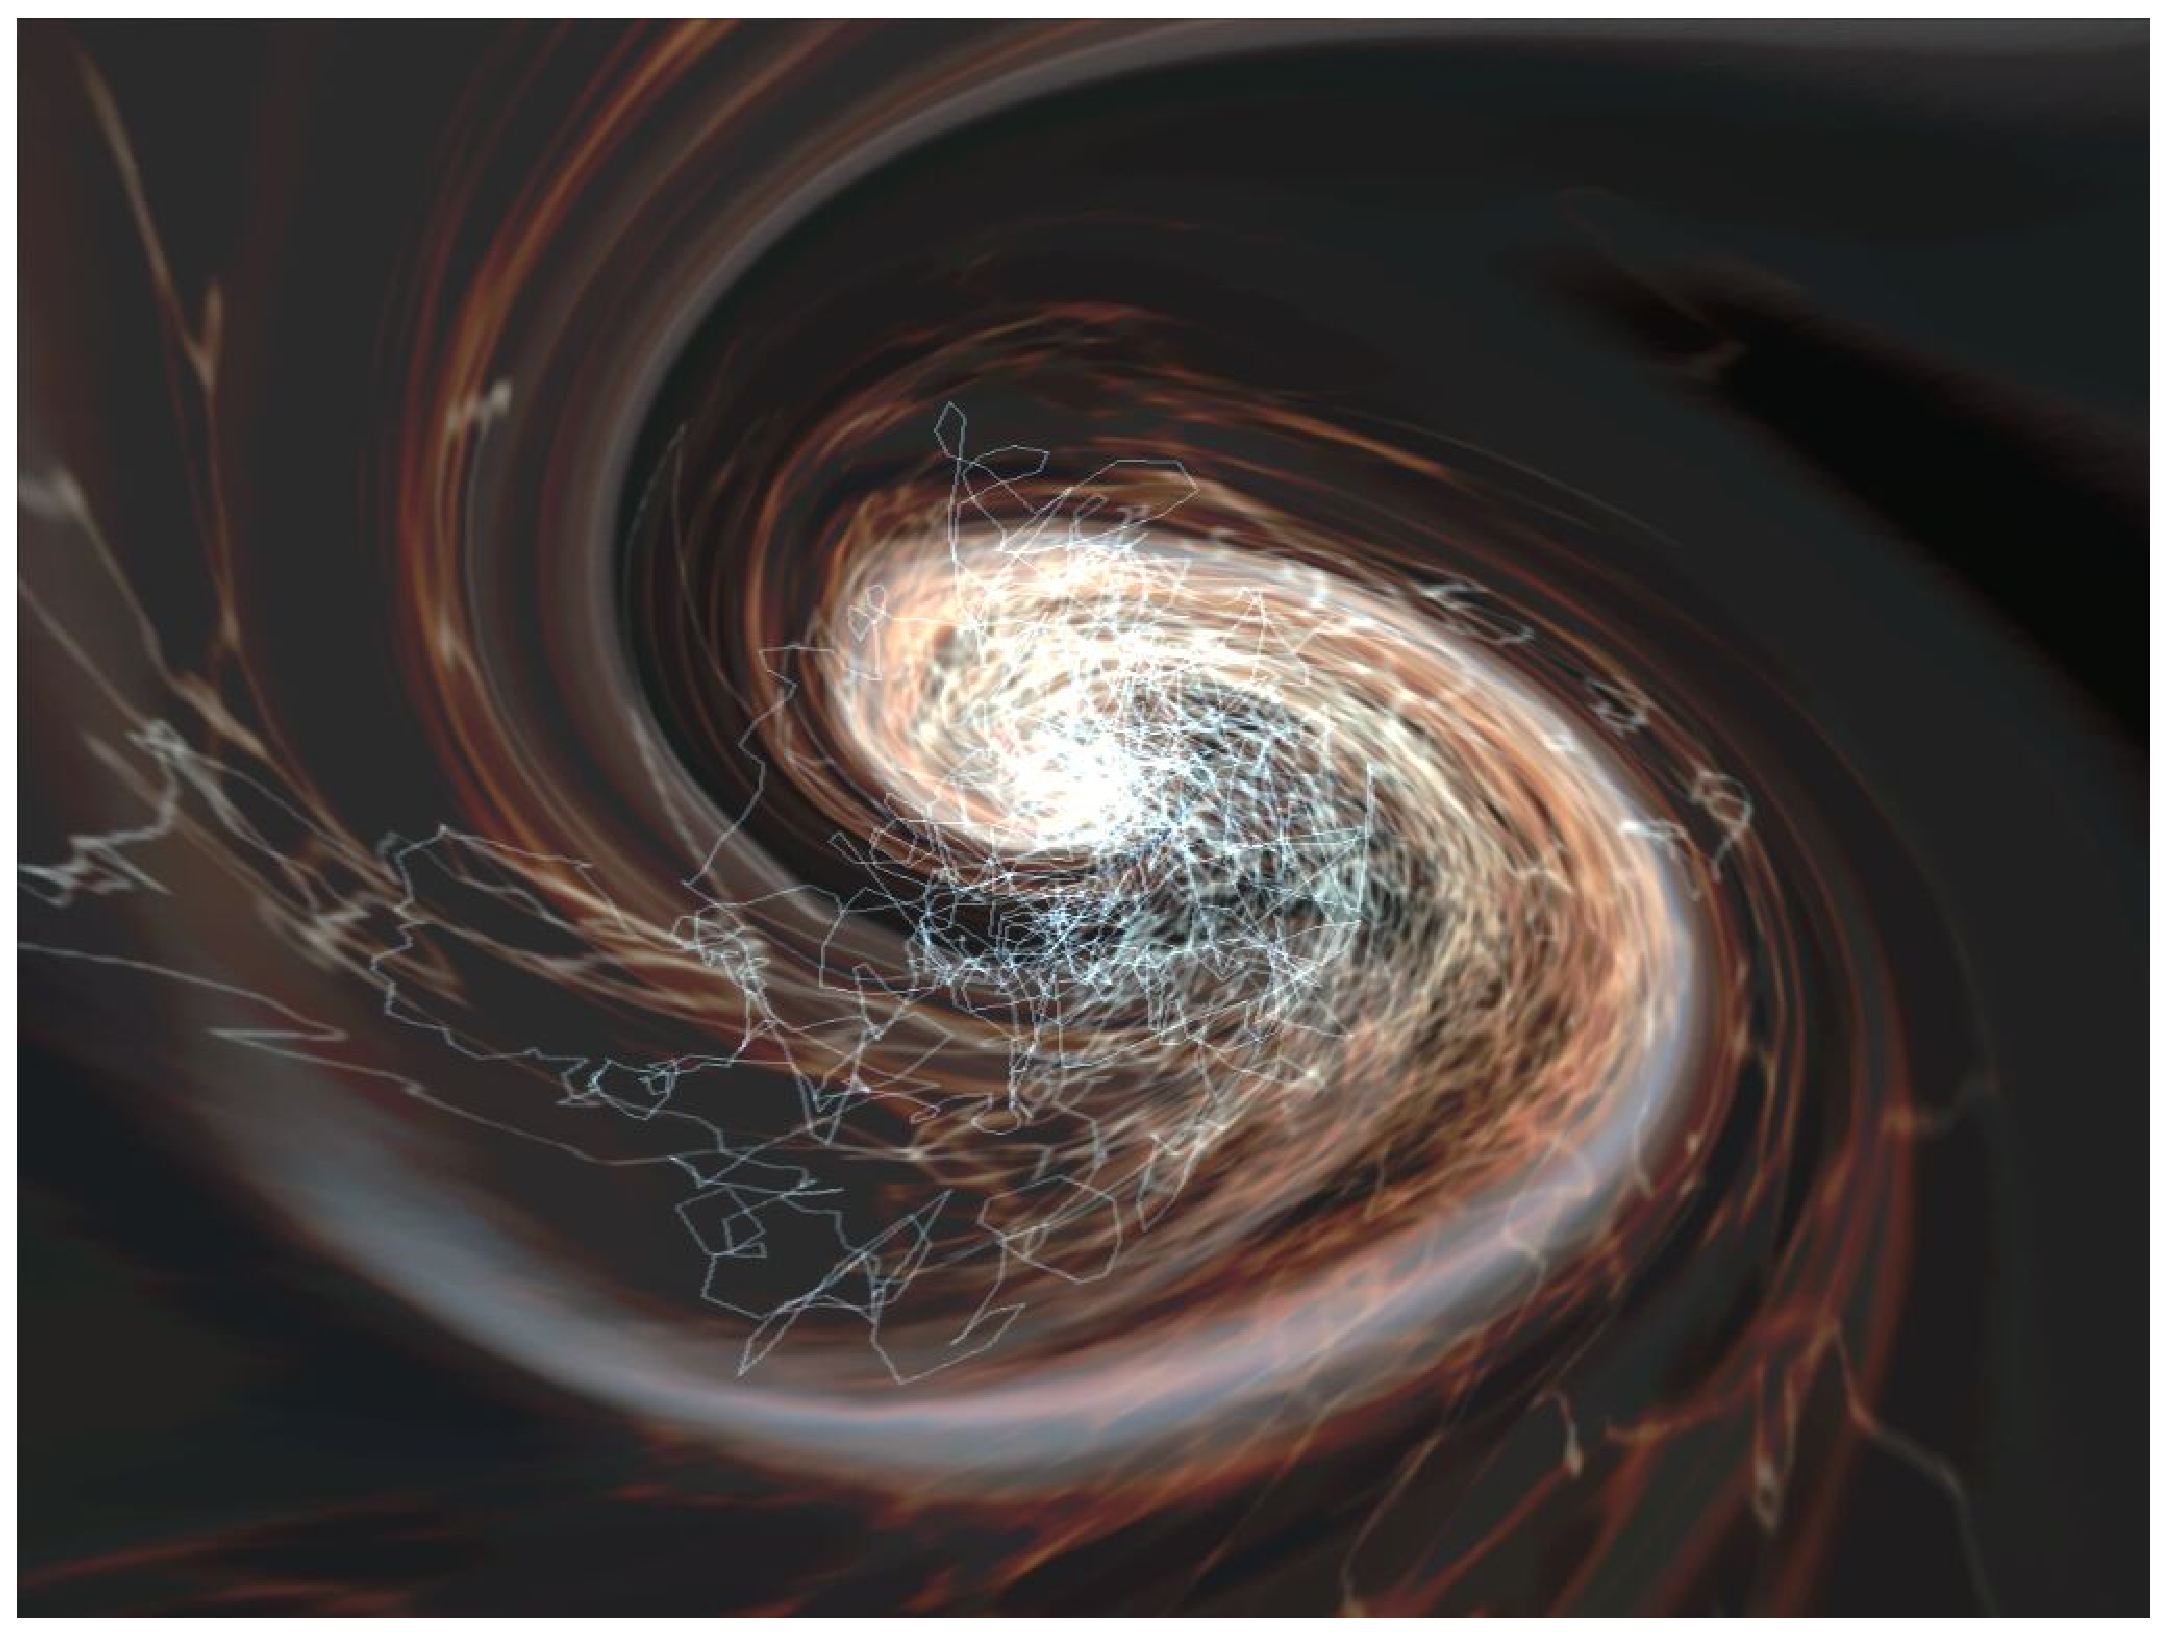
\includegraphics[height=58mm]{milkdrop3.eps}
  \end{figure}
}

\subsection{Open Hardware, for real}
\frame
{
  \frametitle{Open Hardware, for real}

  \begin{itemize}
  \item Arduino = AVR + power supply + connectors.
  \item The AVR chip does all the magic! And it's a black box in every sense.
  \item Here, all the logic of the chip is described (in Verilog HDL)...
  \item ...and open source!
  \item Ask Atmel for the same!
  \end{itemize}
}

\frame
{
  \frametitle{Truly Open Hardware projects}

  \begin{itemize}
  \item GRLIB/LEON3 (Aeroflex Gaisler, ESA)
  \item OpenSPARC (Sun Microsystems)
  \item Open Graphics
  \item OpenPattern
  \item Project VGA
  \item ...and others
  \end{itemize}
}

\section{How is MilkDrop working?}
\frame
{
  \frametitle{How is MilkDrop working?}

Iterative rendering:
  \begin{itemize}
  \item Take the current image, and distort it
  \begin{itemize}
    \item zoom
    \item rotation
    \item scaling
    \item others...
  \end{itemize}
  \item Draw waves and shapes
  \item (In Milkymist: overlay some live video)
  \item Display the result
  \item Repeat the process!
  \end{itemize}
  (This is very simplified)
}

\frame
{
  \frametitle{How is MilkDrop working?}

  \begin{itemize}
  \item Distortion and waves are controlled by fully customizable equations
  \item The set of those equations is called a ``preset''
  \item Similar to a ``patch'' in PureData
  \item Interaction of the visuals with sound is defined by those equations
  \item ...and also with DMX and MIDI in Milkymist
  \end{itemize}
}

\section{Challenges}

\frame
{
  \frametitle{Challenges}

  \begin{itemize}
  \item The need for a CPU
  \begin{itemize}
     \item flexibility
     \item ease of reprogramming
     \item ease of patching software bugs
     \item software-friendly tasks: GUI, filesystems, protocols, ...
  \end{itemize}
  \item FPGA speed, size, and cost
  \begin{itemize}
     \item careful design
     \item balance between hardware and software
     \item software is cheap and slow, hardware is expensive and fast
  \end{itemize}
  \item Memory problems: bandwidth, size
  \item Compute-intensive operations
  \begin{itemize}
     \item distorting the image
     \item evaluating the equations
  \end{itemize}
  \end{itemize}
}

\section{System architecture}
\frame
{
  \begin{center}
  \framebox[100mm][c]{System architecture}
  \end{center}
}

\frame
{
  \frametitle{It contains a microcontroller!}
  \begin{figure}[H]
  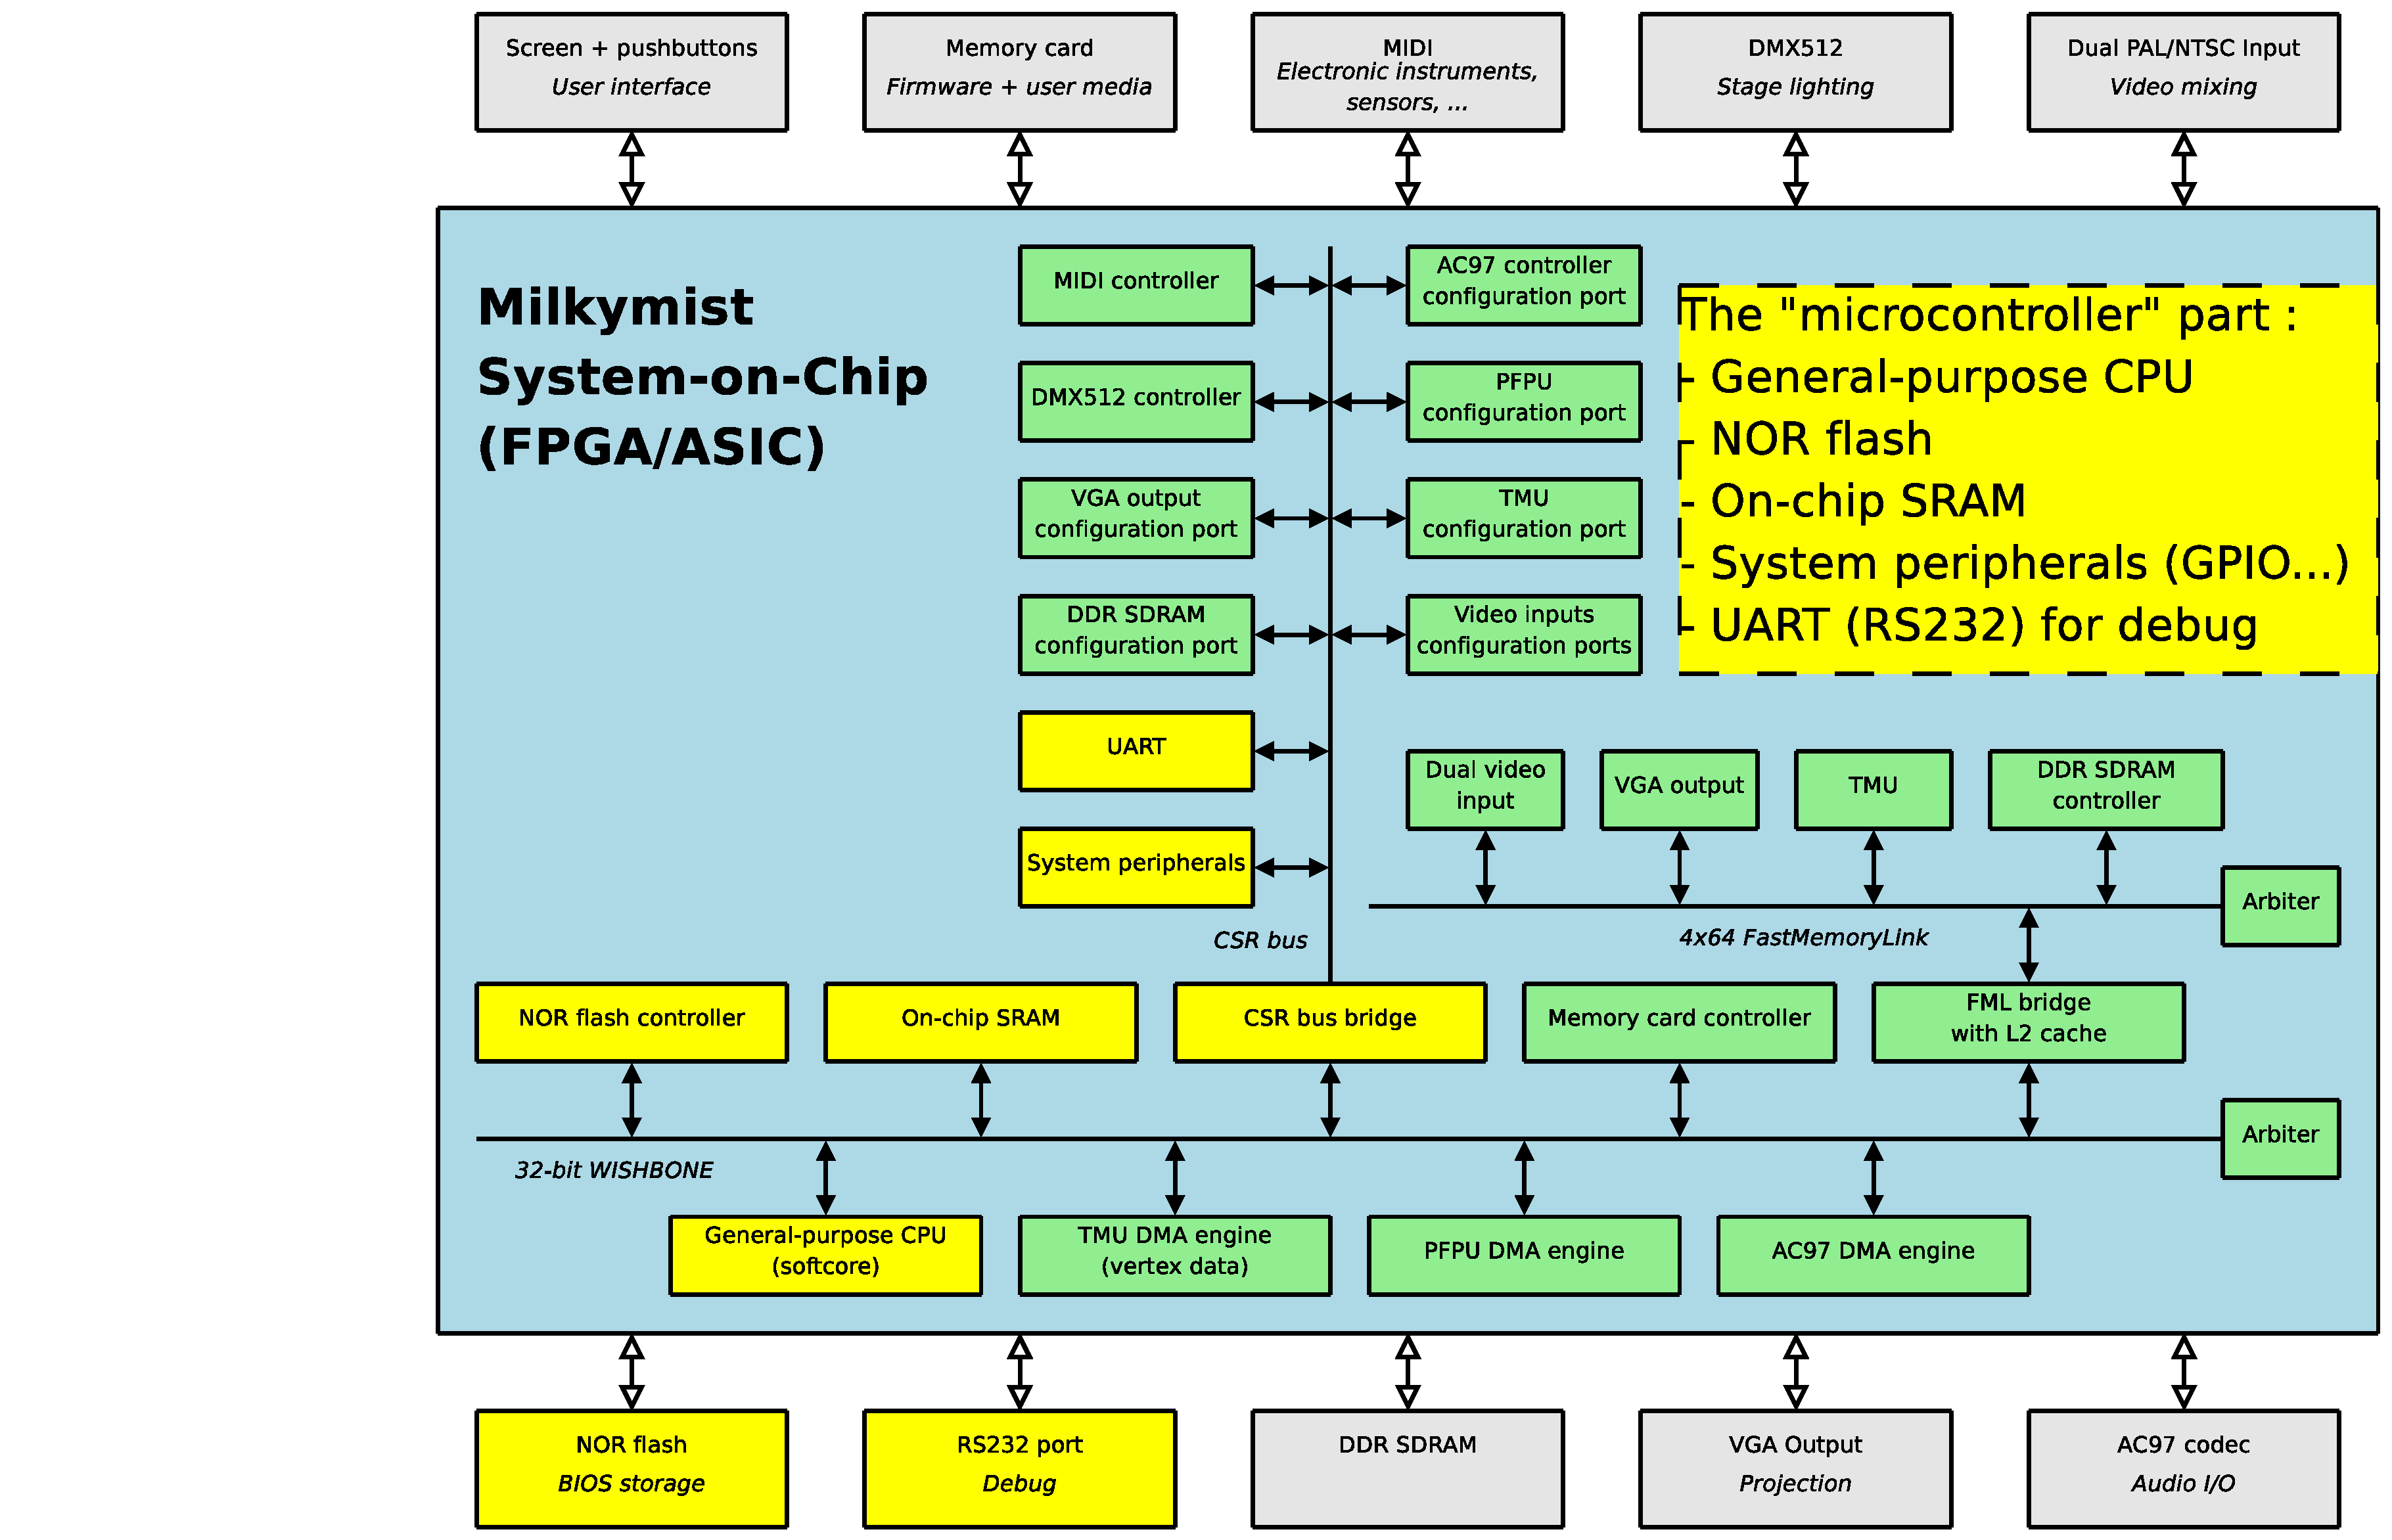
\includegraphics[height=60mm]{microcontroller.eps}
  \end{figure}
}

\frame
{
  \frametitle{The design flow}
  
  ``System-on-a-Programmable-Chip'' (SoPC):
  \begin{itemize}
  \item A microcontroller is implemented using the FPGA fabric
  \item The software is written and compiled (GCC)
  \item The compiled firmware is flashed/loaded on the board
  \item The microprocessor made from the FPGA fabric executes it
  \item Acceleration units and specialty peripherals are added to the system and driven by the software
  \end{itemize}
}

\section{Case studies}

\subsection{The memory problem}
\frame
{
  \begin{center}
  \framebox[100mm][c]{Case studies --- The memory problem}
  \end{center}
}

\frame
{
  \frametitle{The memory problem}
  
  \begin{itemize}
  \item A tough one.
  \item The application requires memory to be big, fast, and cheap at the same time.
  \item The required memory size prohibits the use of SRAM
  \item ...then we have to use DRAM and face all its problems.
  \end{itemize}
}

\frame
{
  \frametitle{How bad is it?}
  
  \begin{tabular}{|l|l|l|}
  \hline
  \textbf{Task} & \textbf{Bandwidth} & \textbf{Capacity} \\
  \hline
  VGA framebuffer, 1024x768, 75Hz, 16bpp & 900Mbps & 3MB \\
  \hline
  Distortion, 1024x768, 30fps, 16bpp & 720Mbps & -- \\
  \hline
  2xNTSC input, 720x576, 30fps, 16bpp & 380Mbps & 3MB \\
  \hline
  Software and misc. & 250Mbps & 16MB \\
  \hline
  \textbf{Total} & \textbf{2.2Gbps} & \textbf{22MB} \\
  \hline
  \end{tabular}\\
  
  \begin{itemize}
  \item One DDR SDRAM chip running at 100MHz:\\(DDR-200 in marketingspeak)
  \begin{itemize}
  \item 3Gbps \underline{peak bandwidth}
  \item 32MB capacity
  \item a few dollars
  \end{itemize}
  \item This is still manageable!
  \end{itemize}
}

\frame
{
  \frametitle{Peak bandwidth?}
  
  Performance of SDRAM depends a lot on the cleverness of its controller. Example:
  
  \begin{figure}[H]
  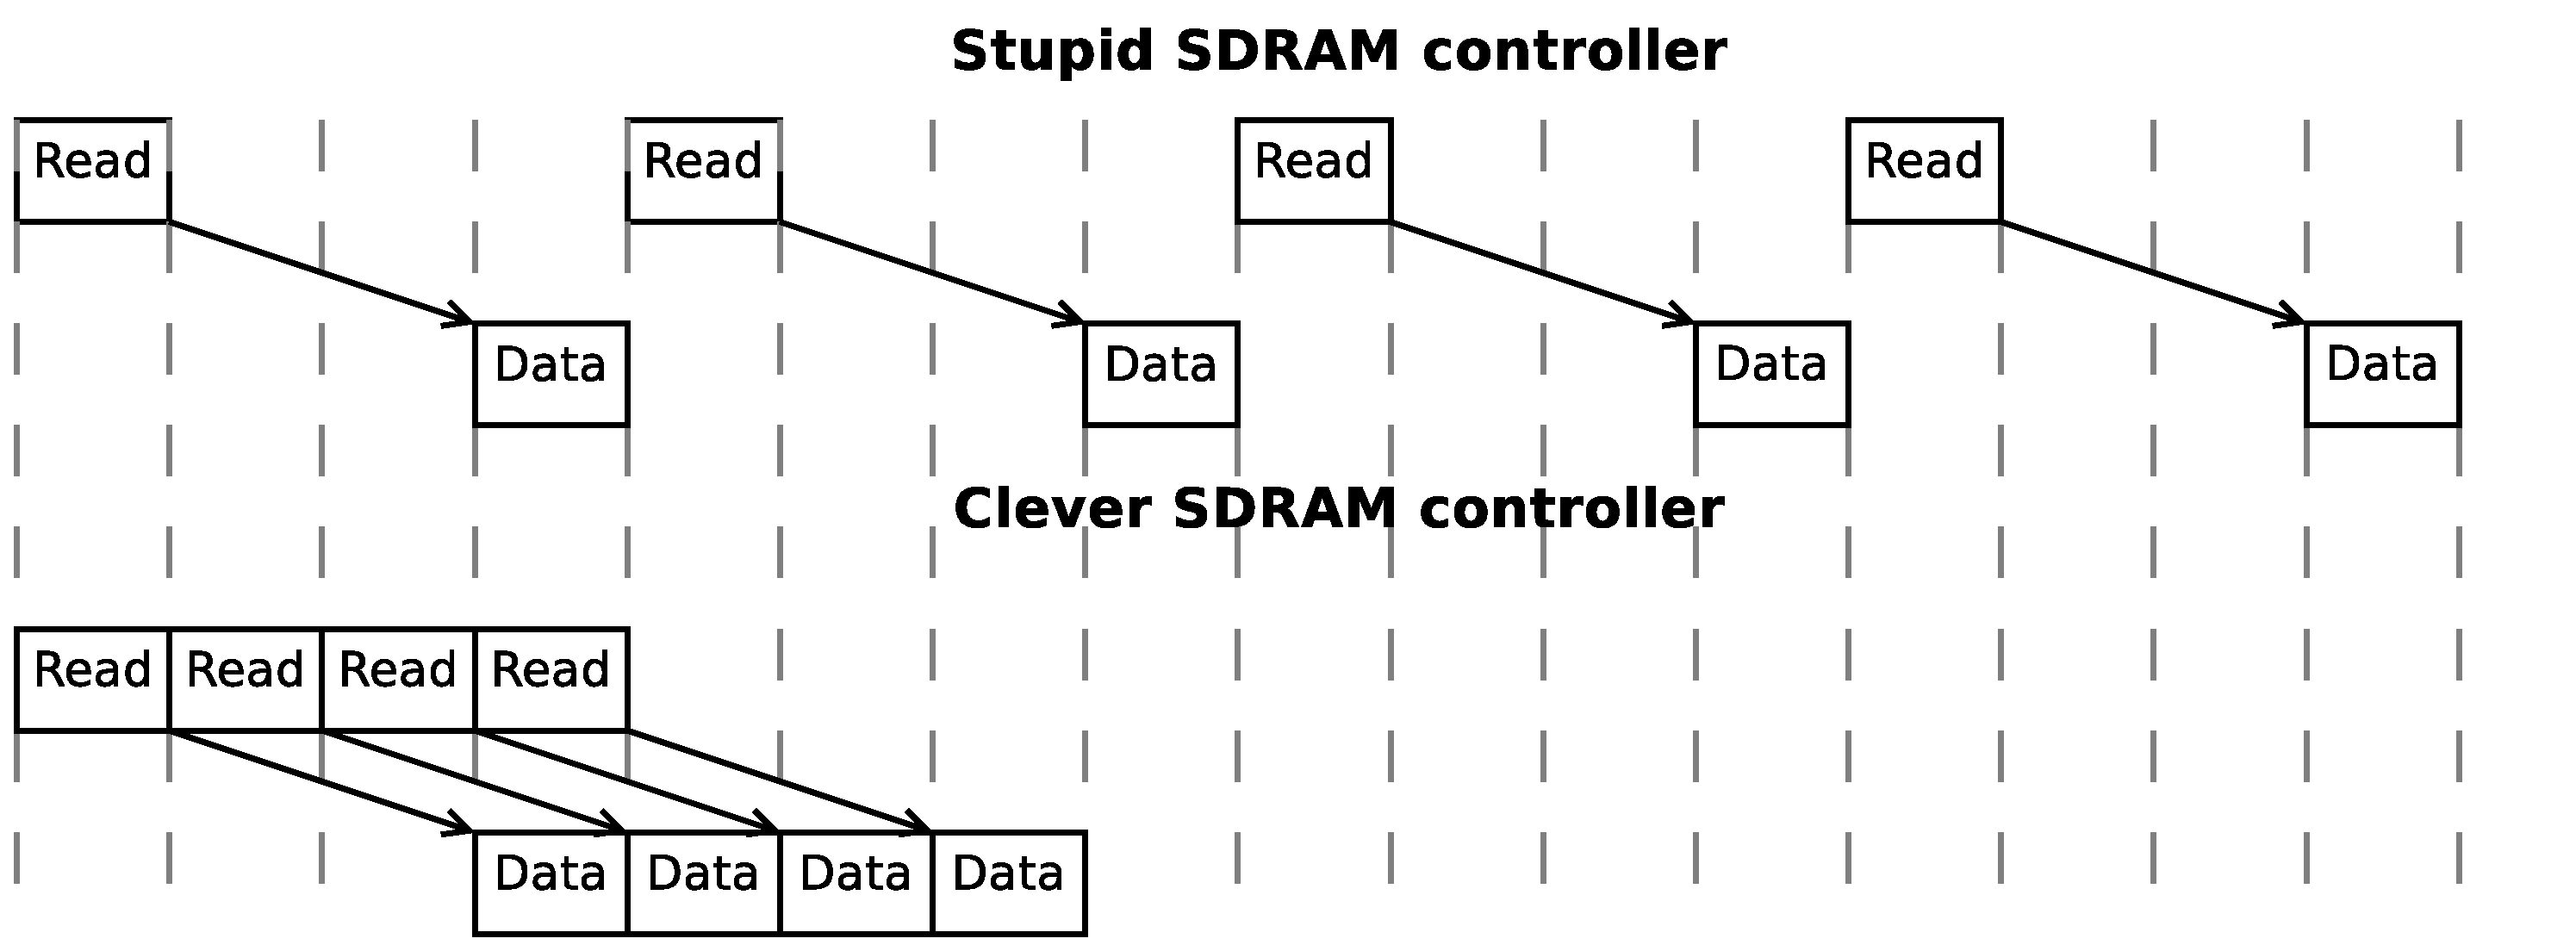
\includegraphics[height=30mm]{memlatency.eps}
  \end{figure}
  
  In Milkymist, memory transfers are always done using bursts of 4 consecutive words (FML bus). The bus master caches or discards the data it does not want.
}

\frame
{
  \frametitle{Bursts of 4 consecutive words: a good heuristics?}
  
  \begin{itemize}
  \item Good for the VGA framebuffer (a big bandwidth consumer):
  \begin{itemize}
  \item when it gets a burst of 4 consecutive chunks from memory...
  \item those chunks also represent consecutive pixels (in scan order)
  \item ...so it can just put them in its output FIFO and easily acheive 100\% utilization!
  \end{itemize}
  \item It is the same for PAL/NTSC video inputs.
  \item For image distortion: yes; more on this later.
  \item For software: principle of temporal/spatial locality, caches.
  \item And simplifies a lot (compared to a variable burst length):
  \begin{itemize}
  \item SDRAM controller design
  \item Bus signaling
  \item Bus arbitration
  \item Cache controllers
  \end{itemize}
  \end{itemize}
}

\subsection{Distorting the image}
\frame
{
  \begin{center}
  \framebox[100mm][c]{Case studies --- Distorting the image}
  \end{center}
}


\frame
{
  \frametitle{What is ``distortion''?}
  
  \begin{figure}[H]
  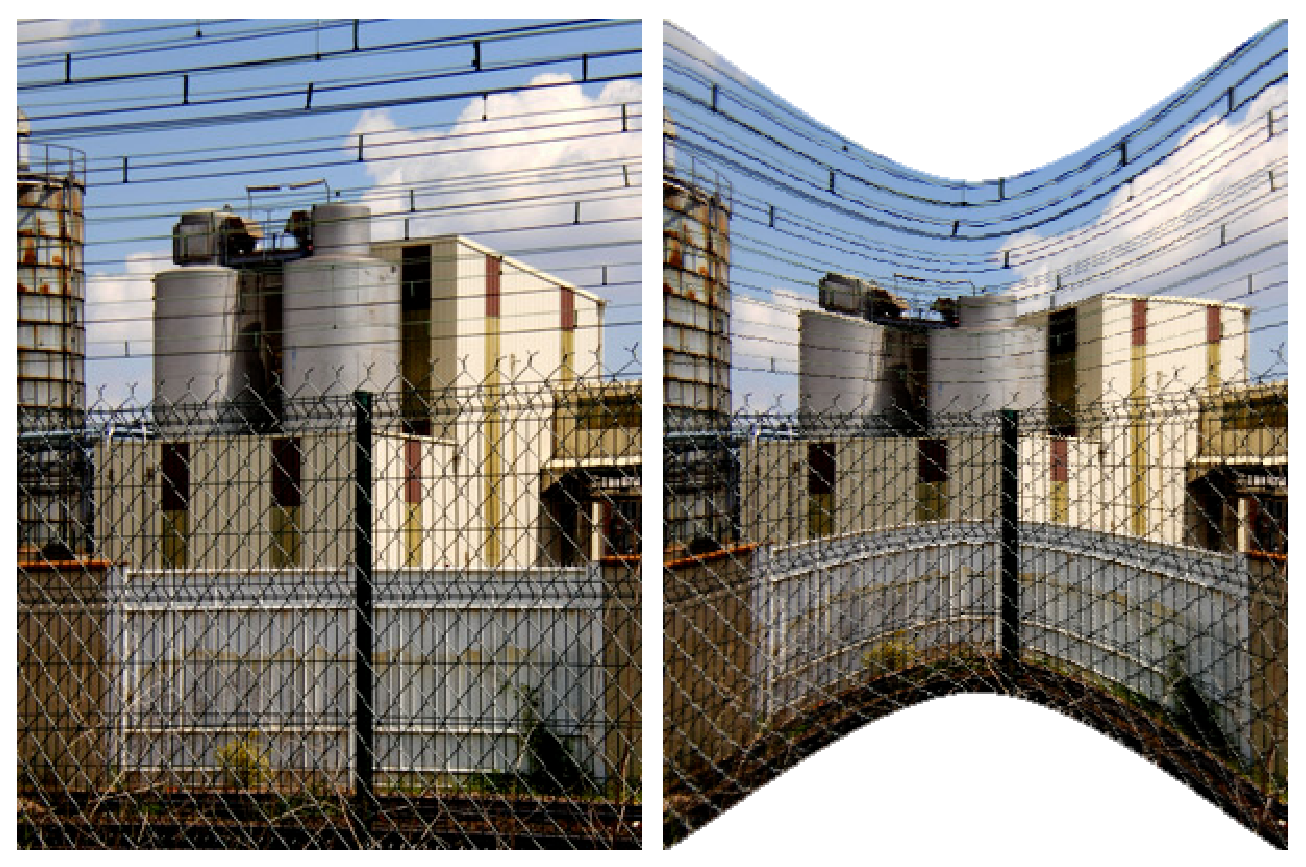
\includegraphics[height=40mm]{distortionsanofi.eps}
  \end{figure}
}

\frame
{
  \frametitle{More precisely...}
  
  \begin{itemize}
  \item ``Texture mapping'' in OpenGL terminology
  \item The MilkDrop preset equations define a mapping $f : (x,y)\rightarrow(X,Y)$
  \item The point at $(x,y)$ in the source image should be at $(X,Y)$ in the destination image
  \item Example: zoom by a factor of 2: $f(x,y) = (2 \cdot x, 2 \cdot y)$
  \item Problem with pixels: how to fill the ``holes''?!
  \item Tessellation, triangle strip
  \end{itemize}
}

\frame
{
  \frametitle{More precisely...}
  \begin{itemize}
  \item Tessellate the source image with triangles.
  \item Apply the mapping to the vertices.
  \item Fill the ``distorted'' triangles in the destination picture.
  \item Interpolate linearly the source coordinates.
  \end{itemize}
  
  \begin{figure}[H]
  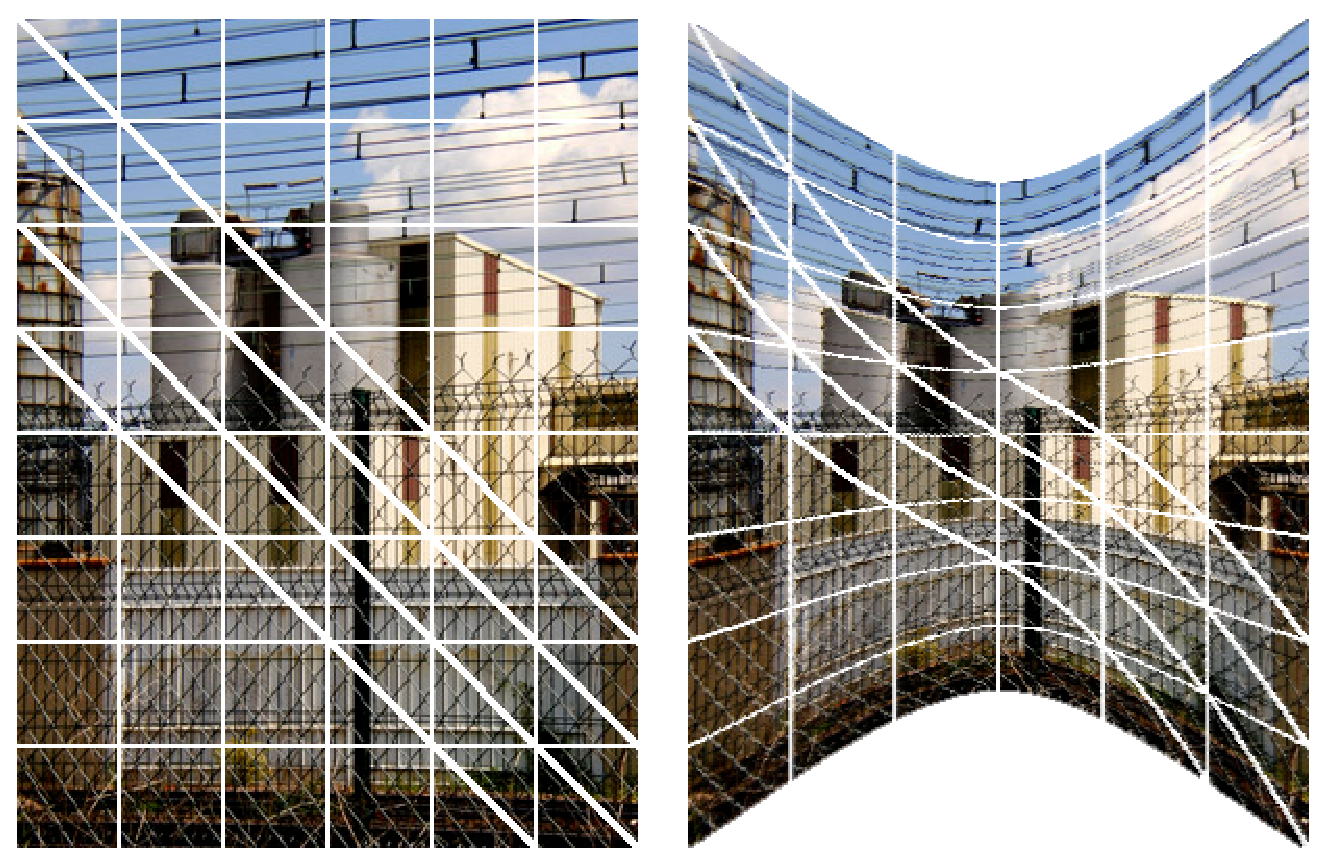
\includegraphics[height=35mm]{tesselsanofi.eps}
  \end{figure}
}

\frame
{
  \frametitle{Performance constraints}
  
  \begin{itemize}
  \item To acheive 30fps at 1024x768, the Texture Mapping Unit (TMU) must process 24 million pixels per second.
  \item With a 100MHz clock, we have 4 cycles to process a pixel.
  \item With a naive implementation, each pixel requires (approx.):
  \begin{itemize}
  \item math: $\approx100$ cycles
  \item one memory read: $\approx12$ cycles
  \item one memory write: $\approx12$ cycles
  \end{itemize}
  \item Total: $\approx124$ cycles!!! Solutions for a $\approx3000\%$ speedup?!?
  \end{itemize}
}

\frame
{
  \frametitle{Solutions}
  
  \begin{itemize}
  \item Improved algorithm
  \begin{itemize}
  \item Bresenham's linear interpolation algorithm
  \end{itemize}
  \item SIMD parallelism
  \begin{itemize}
  \item the same operation on independent data can be done in parallel
  \item example: computing X and Y in the source image
  \end{itemize}
  \item Pipelined parallelism
  \begin{itemize}
  \item Milkymist's TMU has 14 pipeline stages
  \item will grow as more features are added...
  \item commercial GPUs can have hundreds
  \end{itemize}
  \item Smart memory access
  \begin{itemize}
  \item cache
  \item write buffer
  \end{itemize}
  \end{itemize}
}

\frame
{
  \frametitle{Solutions}
  
  \begin{itemize}
  \item Let's focus on the memory read problem.
  \begin{itemize}
  \item others would need deep explanations of the algorithms.
  \end{itemize}
  \item Currently takes $\approx12$ cycles, and we have at most 4.
  \item Use the bursts, and memorize them in a cache.
  \end{itemize}
  \begin{figure}[H]
  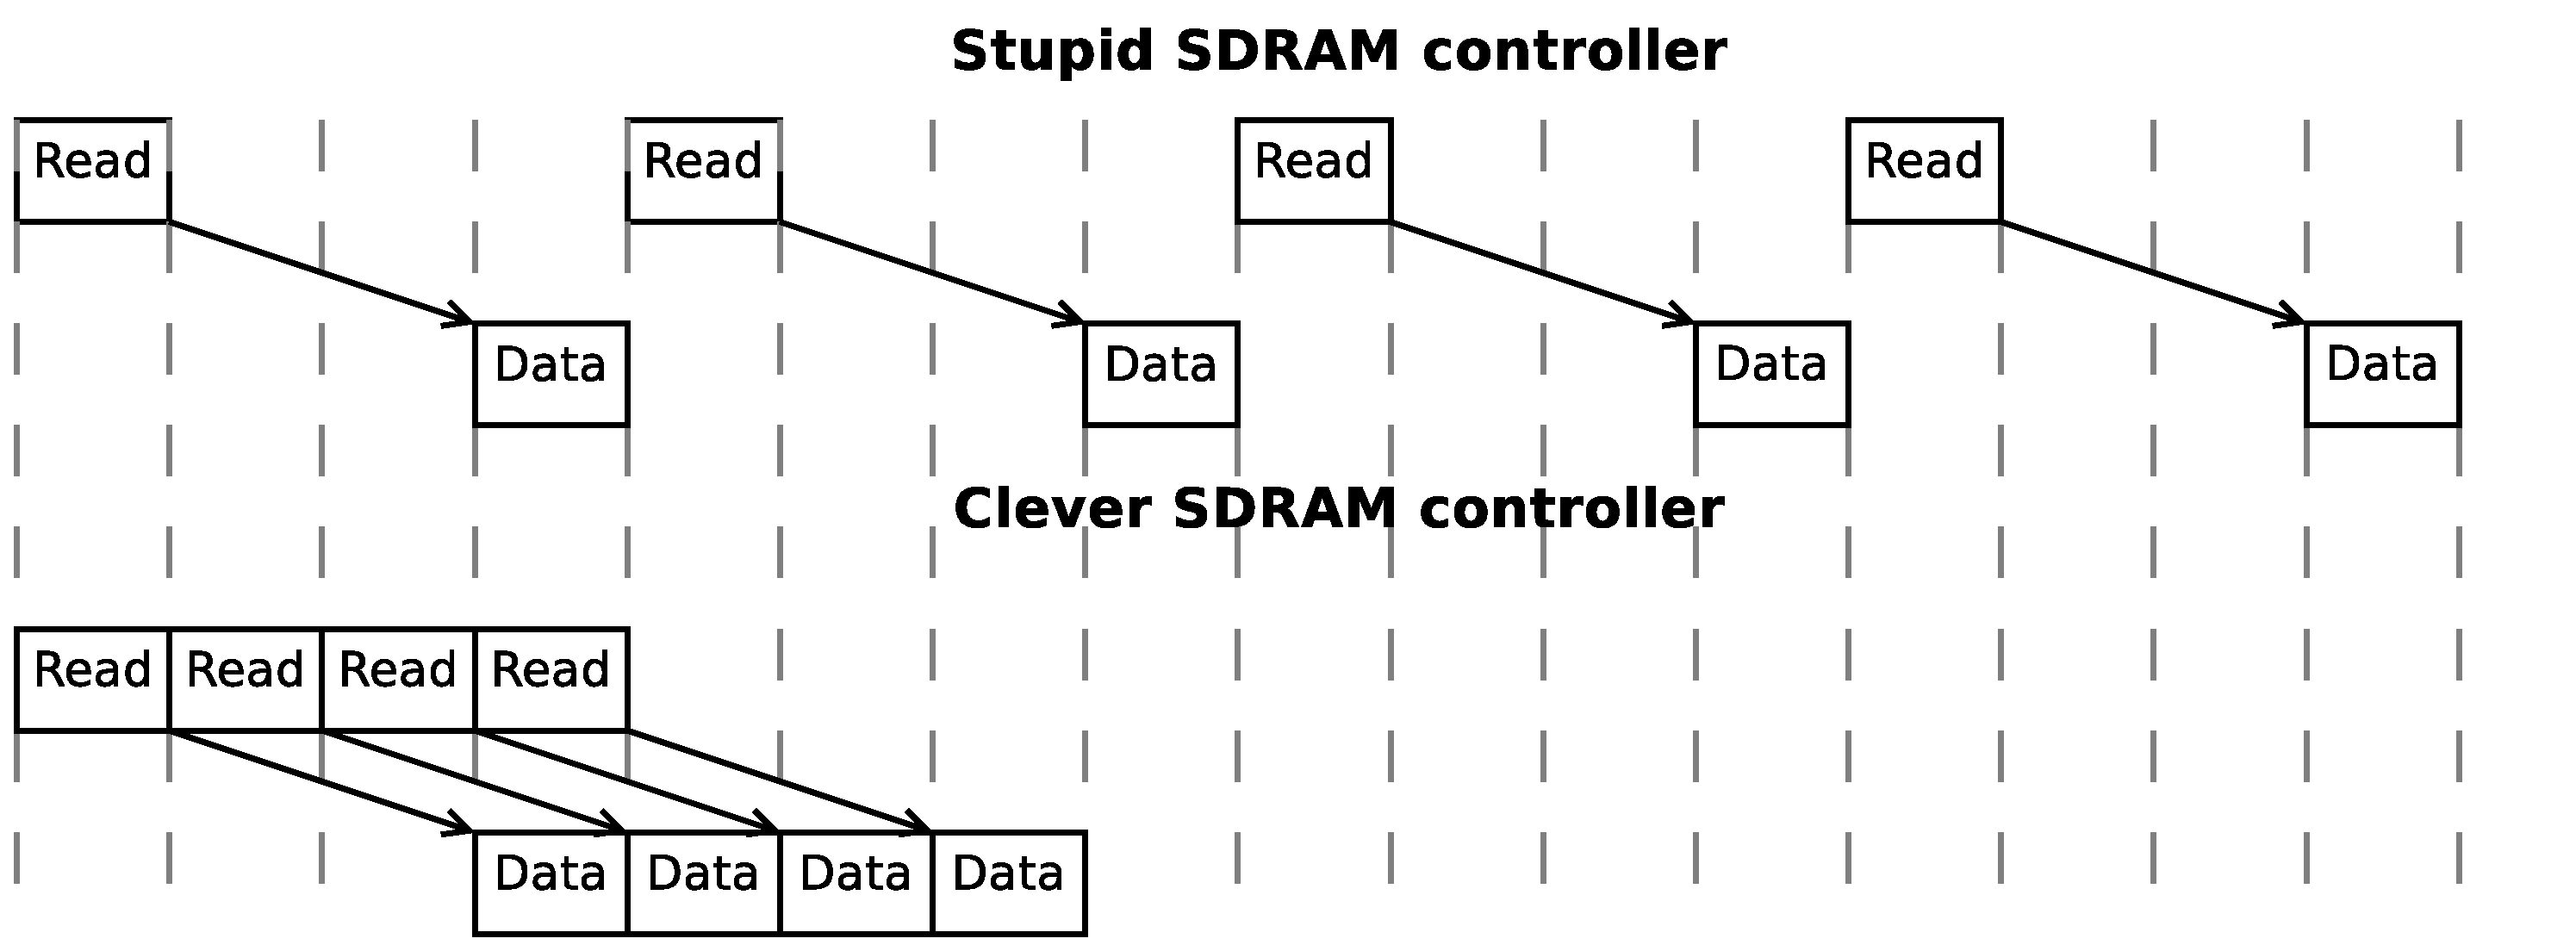
\includegraphics[height=30mm]{memlatency.eps}
  \end{figure}
}

\frame
{
  \frametitle{Are bursts and cache a good idea?}
  
  Example: rotation of a triangle.
  \begin{figure}[H]
  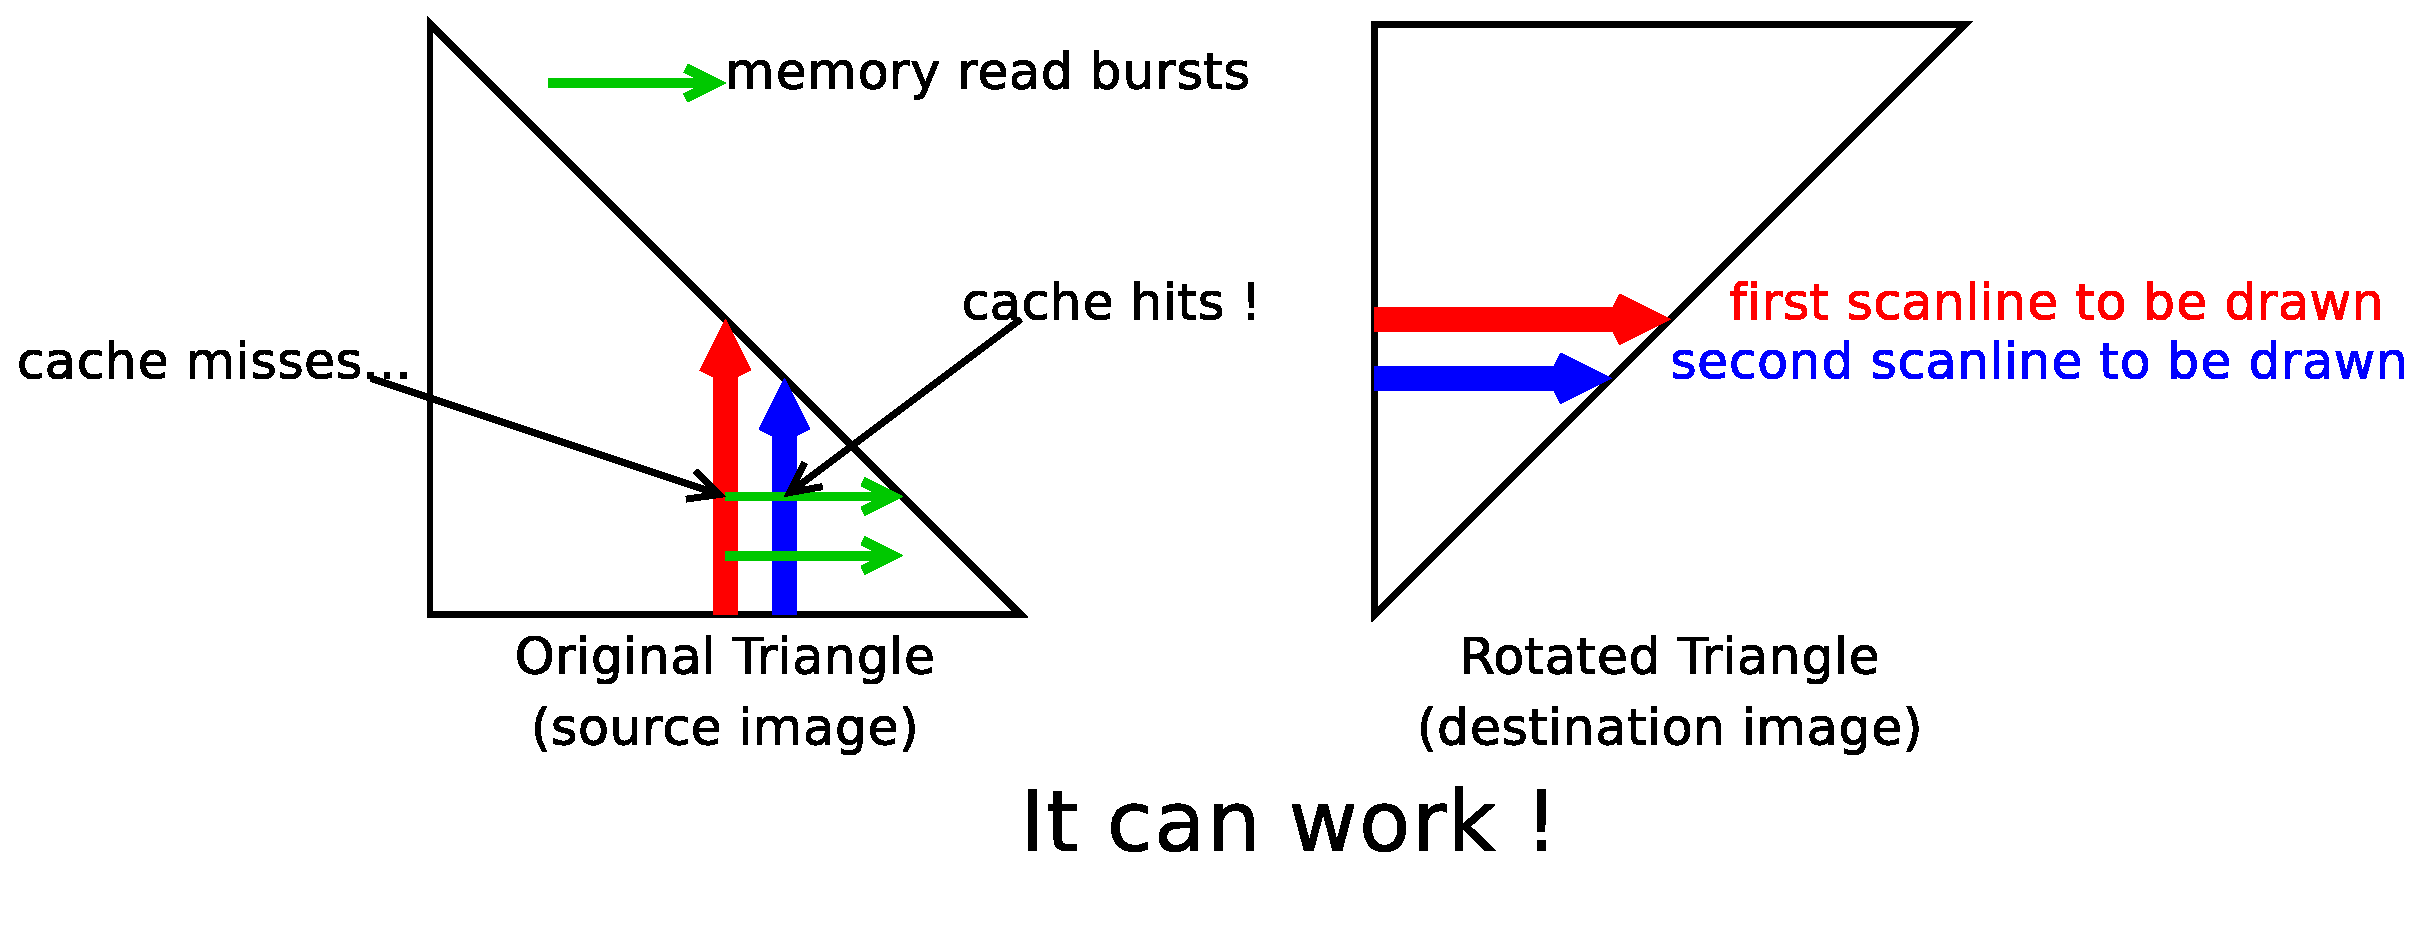
\includegraphics[height=40mm]{tripattern.eps}
  \end{figure}
}

\frame
{
  \frametitle{How big should the cache be?}
  \begin{figure}[H]
  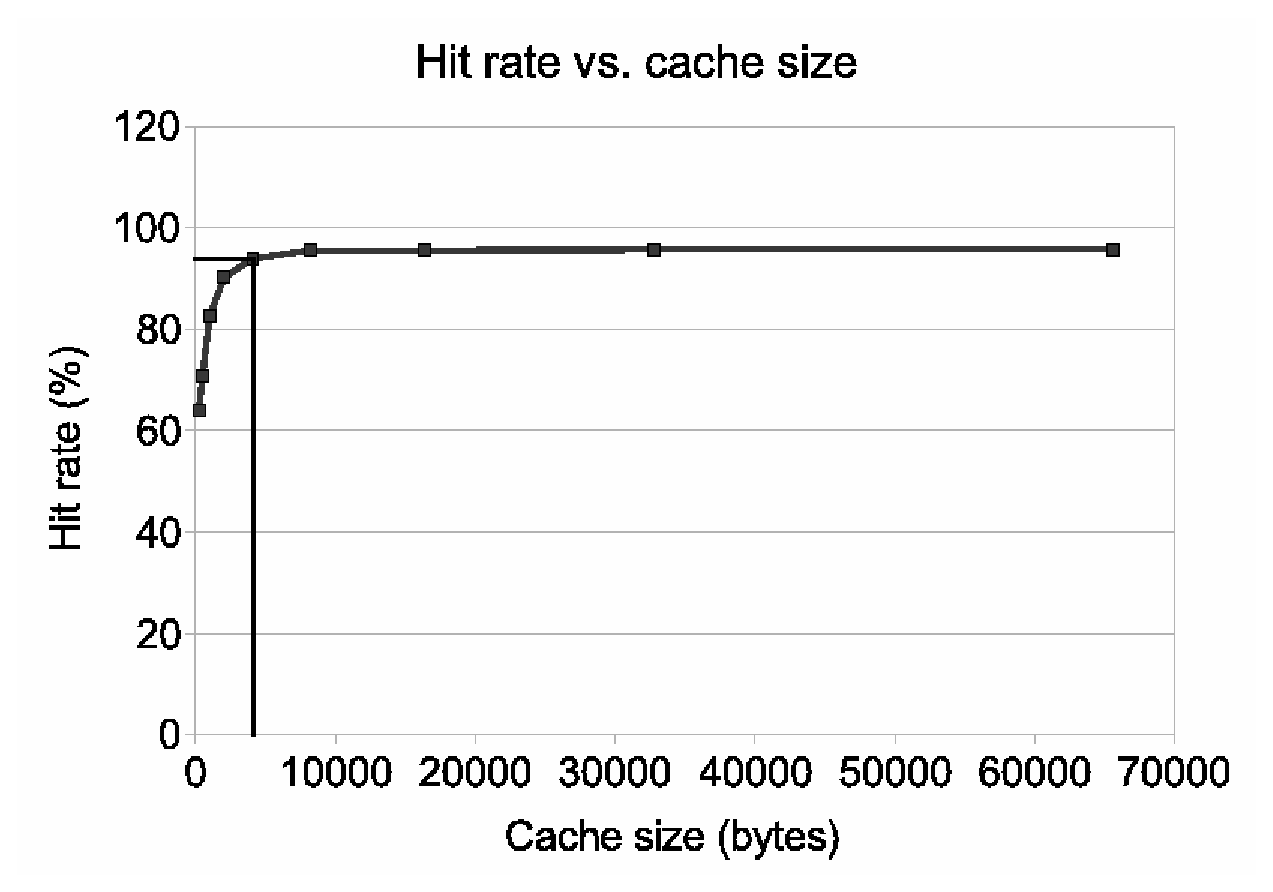
\includegraphics[height=38mm]{texelcache.eps}
  \end{figure}
  \begin{itemize}
  \item Cache size: 4KB
  \item Hit rate: 94\%
  \item Average memory access time: 1.4 cycles
  \item Problem solved!
  \end{itemize}
}

\subsection{Evaluating MilkDrop equations}
\frame
{
  \begin{center}
  \framebox[100mm][c]{Case studies --- Evaluating MilkDrop equations}
  \end{center}
  \begin{itemize}
  \item Some performance tricks are also used here
  \item Floating-point hardware coprocessor (PFPU)
  \item The main CPU compiles code on-the-fly for the coprocessor
  \end{itemize}
}

\section{In practice}
\frame
{
  \begin{center}
  \framebox[100mm][c]{In practice}
  \end{center}
}

\subsection{Development hardware}
\frame
{
  \frametitle{Development board}
  \begin{itemize}
  \item Most developments were done on a Xilinx ML401 board.
  \item Feature-rich.
  \item Affordable: $\approx\$500$.
  \end{itemize}
  \begin{figure}[H]
  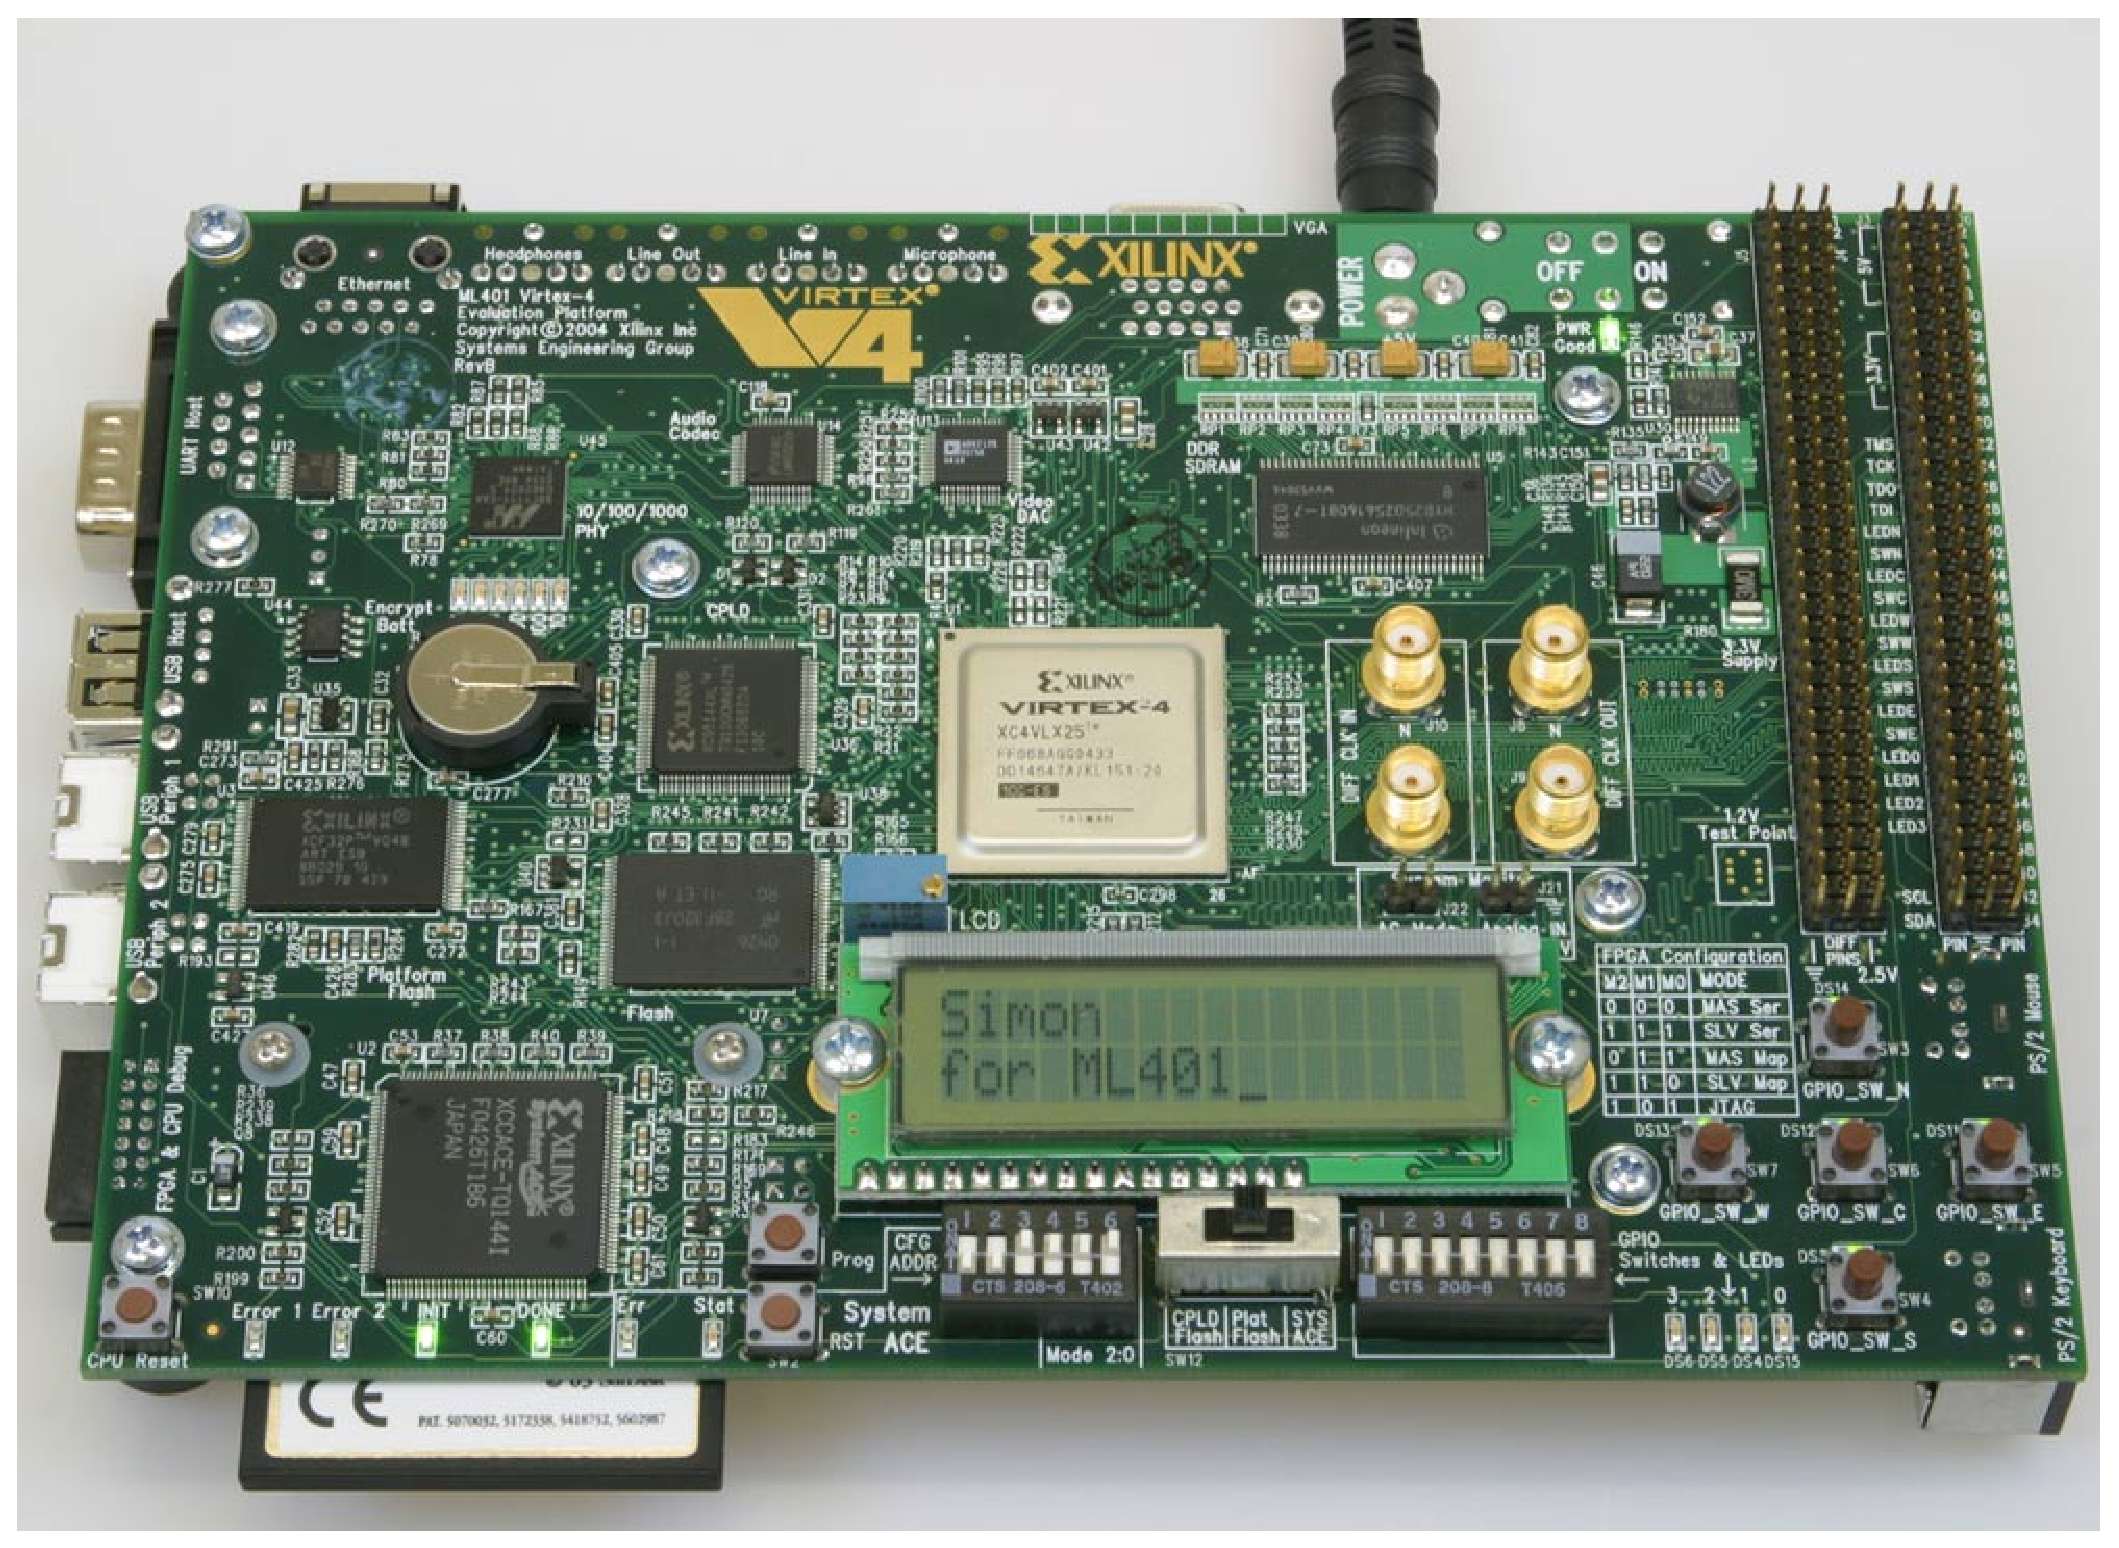
\includegraphics[height=40mm]{ml401.eps}
  \end{figure}
}


\subsection{Development software}
\frame
{
  \frametitle{Verilog simulations}
  \begin{itemize}
  \item Free simulators
  \begin{itemize}
  \item Icarus Verilog
  \item GPL Cver
  \item Verilator, innovative and amazingly fast, but currently buggy
  \end{itemize}
  \item Light-weight, run without a hitch on ultra-mobile laptops (EeePC)
  \begin{itemize}
  \item debug your Verilog code anytime and anywhere
  \item try to do the same with Modelsim and FLEXnet licensing!
  \end{itemize}
  \item Expensive proprietary simulators from big EDA companies were not needed to develop Milkymist.
  \end{itemize}
}

\frame
{
  \frametitle{Logic synthesis}
  \begin{itemize}
  \item ISE Webpack from Xilinx.
  \item Proprietary but free of charge.
  \item Linux version.
  \item Pretty good quality if you stick to command line.
  \end{itemize}
}

\frame
{
  \frametitle{Software development}
  \begin{itemize}
  \item CPU is supported by the GCC compiler (C/C++).
  \item For debugging, software can be downloaded from RS232.
  \end{itemize}
  \begin{figure}[H]
  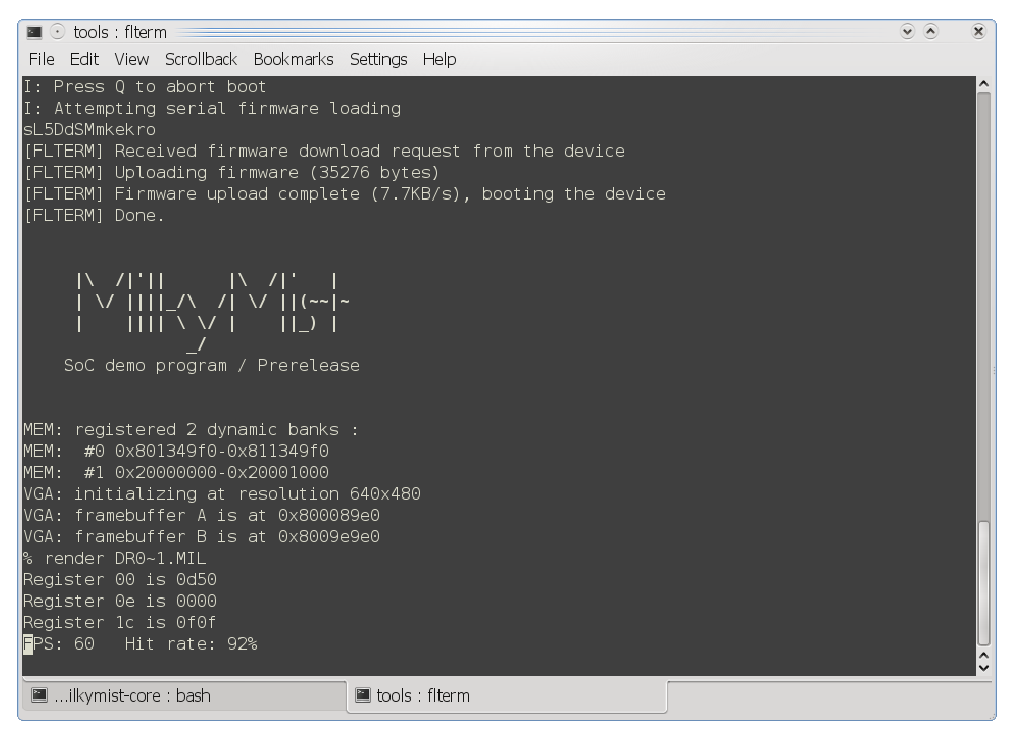
\includegraphics[height=45mm]{serialdebug.eps}
  \end{figure}

}


\section{Conclusion}
\frame
{
  \frametitle{Conclusion}
  \begin{itemize}
  \item Wide availability of FPGAs opens new fields for hobbyists.
  \item High-speed embedded computing, and applications.
  \item This talk has presented a couple of high-performance logic design techniques.
  \item I did not invent them. They are ubiquitous in the computer industry, but seldom heard of.
  \end{itemize}
}

\frame
{
  \frametitle{Thank you for your attention}
  \begin{itemize}
  \item Web: \url{http://www.milkymist.org}
  \begin{itemize}
  \item documented source code (GPLv3 licensing)
  \item binary kits (to get started fast)
  \item mailing list
  \item wiki (with suggested contributions)
  \item blog
  \item these slides are online
  \end{itemize}
  \item Mail: sebastien.bourdeauducq [AT] lekernel DOT net
  \end{itemize}

  \begin{center}
  \framebox[100mm][c]{Questions?}
  \end{center}
}

\end{document}
